\chapter{Chapter 6 : Final Tic-Tac-Toe Software}

For the software component of the Tic-Tac-Toe game, a web application will be used to make the moves. This web app will communicate with a backend system, which will then interface with the microcontroller to control the coils that move the game pieces.

\section{Web App - Frontend}

The web application is straightforward, featuring a 3x3 grid of buttons. When a button is pressed, it sends a request to the backend to execute the move. While the board is making a move, the buttons are temporarily disabled. The web app waits for confirmation from the backend before re-enabling the buttons for the next move.

\begin{figure}[H]
	\centering
	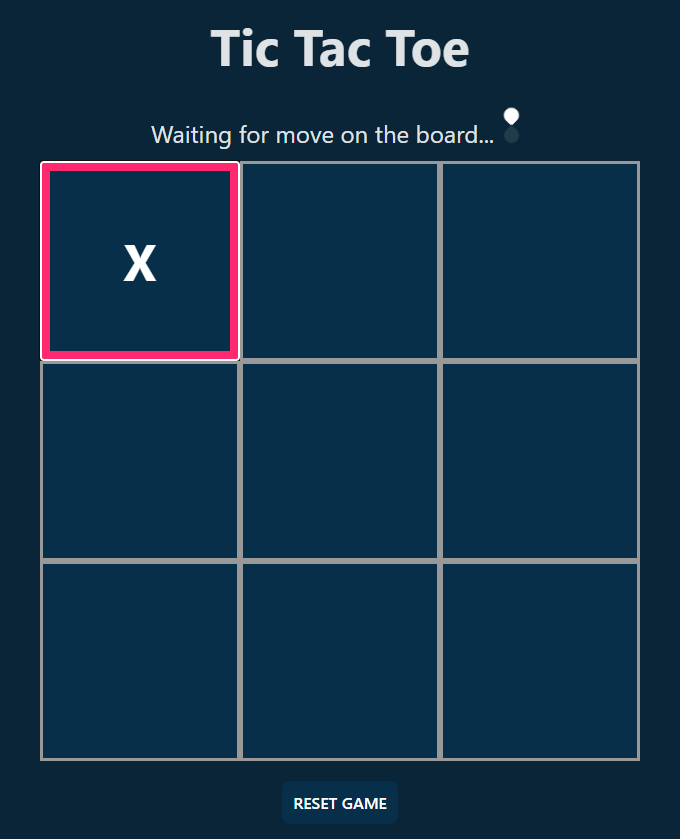
\includegraphics[width=0.6\linewidth]{web_waiting.png}
	\caption[Web app waiting for an acknowledgement after a player move]{Web app waiting for an acknowledgement after a player move}
	\label{fig:web_waiting}
\end{figure}

The web app is made with React.js\footcite{noauthor_react_nodate}, a JavaScript library for building user interfaces. It is a single page application that uses the WebSocket protocol to communicate with the backend.

\section{Web App - Backend}

The backend is a straightforward Python script that establishes a WebSocket connection with the web app. It listens for messages from the web app and forwards them to the microcontroller via serial communication. After receiving an acknowledgment from the microcontroller, the backend sends the result back to the web app.

The serial communication is also simple: the backend sends the move coordinates to the microcontroller, framed by a start byte and a stop byte. Since the frontend handles the game rules and permissions, the backend only receives valid moves, ensuring that no illegal moves are processed.

Packet from the backend to the microcontroller:
\begin{itemize}
	\item Start byte : 0x02
	\item X coordinate : 0 to 2 in ASCII
	\item Y coordinate : 0 to 2 in ASCII
	\item Stop byte : 0x03
\end{itemize}

Packet from the microcontroller to the backend:
\begin{itemize}
	\item Start byte : 0x02
	\item Result : OK or KO in ASCII (KO when issue happened)
	\item Stop byte : 0x03
\end{itemize}

\newpage

\section{Microcontroller firmware}

The RP2040 is programmed in C with the Pico SDK\footcite{noauthor_hardware_nodate} and I decided to use a Real Time Operating System for easier multi task management and timings, I chose FreeRTOS\footcite{noauthor_freertos_nodate}.

The firmware will wait for a packet from the backend, then it will find the best path to move the magnet to the desired position. It will fill a queue with the coils to activate in the correct order. It will then activate the coils one by one and wait some arbitrary time before activating the next coil. When the sequence is done, it will send an acknowledgement to the backend.

The magnets are moved by activating the coils in the correct order. For that, we have to generate a \gls{pwm} signal on the columns and activate the rows.

The RP2040 has an integrated \gls{pwm} peripheral that can be programmed via the Pico SDK API to generate the \gls{pwm} signal.

A simpler API was made to abstract some computing to get the best timer values, so we only have to chose a Frequency and and we can then set a duty cycle from 0.0 to 1.0 when desired.

\begin{figure}[H]
	\centering
	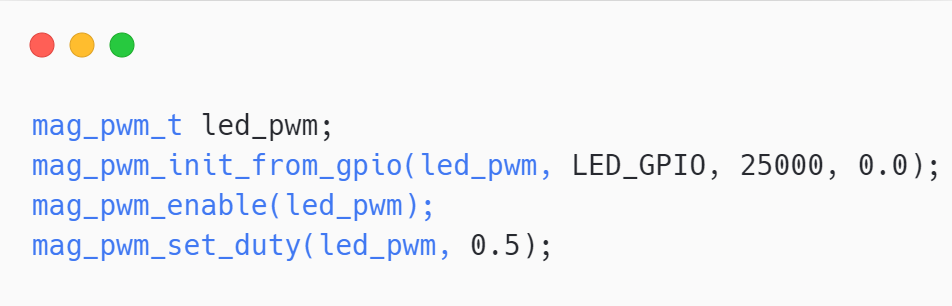
\includegraphics[width=1\linewidth]{code_PWM.png}
	\caption[Custom PWM API]{Custom PWM API}
	\label{fig:pwm_api}
\end{figure}


